\documentclass[10pt, a4paper, italian]{article}
\usepackage[T1]{fontenc}
\usepackage[utf8]{inputenc}
\usepackage{amsmath, amssymb, amsthm, thmtools, amsfonts, mathtools}
\usepackage{nicefrac}
\usepackage{calc}
\usepackage[pdftex, hyperindex, plainpages=false]{hyperref}
\usepackage[nameinlink]{cleveref} %load before classicthesis (clash)
%\usepackage[nochapters,pdfspacing]{classicthesis}
\usepackage{siunitx}
\usepackage[siunitx]{circuitikz}

\usepackage[a4paper]{geometry}
\usepackage{float}
\usepackage{mdframed}
\usepackage{titling}
\usepackage{booktabs}
\usepackage{graphicx}
\usepackage{caption, subcaption}
\usepackage{xcolor}
\usepackage[italian]{babel}
\usepackage{pgfplots}
\usepackage{listings}
%\usepackage{lmodern}
\usepackage{url}
\usepackage{enumitem}
\usepackage{tikz} %loads after classicthesis (xcolor incompat)

% lets graphicx know path where figures to be included are found
\graphicspath{{../figs/}}
\makeatletter
\def\input@path{{../figs/}}
%or: \def\input@path{{/path/to/folder/}{/path/to/other/folder/}}
\makeatother

% tikz pgf plots setup
\usepgfplotslibrary{external}
\pgfplotsset{compat=1.15}
%\tikzexternalize

% spaces and significant digits/figures for measurements
\sisetup{free-standing-units, space-before-unit, number-unit-product = \;,
scientific-notation = false, round-mode = figures, round-precision = 1,}

% turns all (hyperlinked) references black [default is blue]
\hypersetup{
	linktoc=all,
	colorlinks=true,
	linkcolor=black
}

% code listings config
%\lstset{
%language=Python,
%basicstyle=\ttfamily,
%columns=fullflexible,
%keepspaces=true,
%}

% mdframed (for boxed text) configuration
\mdfsetup{linewidth=0.6pt}

% Default fixed font does not support bold face
\DeclareFixedFont{\ttb}{T1}{txtt}{bx}{n}{12} % for bold
\DeclareFixedFont{\ttm}{T1}{txtt}{m}{n}{12}  % for normal

% Custom colors
\usepackage{color}
\definecolor{deepblue}{rgb}{0,0,0.5}
\definecolor{deepred}{rgb}{0.6,0,0}
\definecolor{deepgreen}{rgb}{0,0.5,0}

% Commands 
\newcommand{\executeiffilenewer}[3]{%
	\ifnum\pdfstrcmp{\pdffilemoddate{#1}}%
		{\pdffilemoddate{#2}}>0%
	{\immediate\write18{#3}}\fi%
}
% input .svg --> .pdf_tex graphs
%\newcommand{\includesvg}[1]{%
%	\executeiffilenewer{#1.svg}{#1.pdf}%
%	{inkscape -z -D --file=#1.svg %
%	--export-pdf=#1.pdf --export-latex}%
%	\input{#1.pdf_tex}%
%}
% Thanks UniPi's Department of Physics E. Fermi
\newcommand{\thanksdf}{(\thanks{Dipartimento di Fisica E.~Fermi,%
Universit\`a di Pisa - Pisa, Italy.}\;)}

% hyperlink to email address
\newcommand{\mail}[1]{\href{mailto:#1}{\textsf{#1}}}

% \vec for bold vectors, instead of overarrows (now "\arrvec")
\let\arrvec=\vec
\renewcommand{\vec}[1]{\boldsymbol #1}
% replaces straight phi with slanted phi
\renewcommand{\phi}{\varphi}
% replaces straight eps with curved epsilon
\newcommand{\eps}{\varepsilon}
% abbreviation for (sub_/super^)scripts of \lim, \sum,... in inline math
\newcommand{\ds}{\displaystyle}

% blackboard/number set letters
\newcommand{\CC}{\mathbb C}
\newcommand{\HH}{\mathbb H}
\newcommand{\KK}{\mathbb K}
\newcommand{\NN}{\mathbb N}
\newcommand{\PP}{\mathbb P}
\newcommand{\QQ}{\mathbb Q}
\newcommand{\RR}{\mathbb R}
\newcommand{\ZZ}{\mathbb Z}

\newcommand{\Abs}[1]{{\left\Vert #1\right\Vert}}
\newcommand{\enclose}[1]{{\left( #1 \right)}}
\newcommand{\Enclose}[1]{{\left[ #1 \right]}}
\newcommand{\floor}[1]{\left\lfloor #1 \right\rfloor}
\newcommand{\ceil}[1]{\left\lceil #1 \right\rceil}
\newcommand{\To}{\rightrightarrows}

% Math operators
\DeclareMathOperator{\divergence}{div}
\renewcommand{\div}{\divergence}
\DeclareMathOperator{\Imaginarypart}{Im}
\renewcommand{\Im}{\Imaginarypart}
\DeclareMathOperator{\Realpart}{Re}
\renewcommand{\Re}{\Realpart}
%\DeclareMathOperator{\arg}{arg}
\DeclareMathOperator{\tg}{tg}
\DeclareMathOperator{\arctg}{arctg}
\DeclareMathOperator{\settsinh}{settsinh}
\DeclareMathOperator{\settcosh}{settcosh}
\DeclareMathOperator{\tr}{tr}
\DeclareMathOperator{\im}{im}
\DeclareMathOperator{\sgn}{sgn}
\DeclareMathOperator{\diag}{diag}

\DeclarePairedDelimiter{\norm}{\lVert}{\rVert}
\DeclarePairedDelimiter{\scalar}{\langle}{\rangle}

% Logarithm with arbitrary base.
% -> log_10
\newcommand{\llog}[1][10]{\log_{#1}}

% Absolute value.
% -> |x|
\newcommand{\abs}[1]{\left| #1 \right|}

% Powers.
% -> x^a
\newcommand{\power}[2][2]{\left( #2 \right)^{#1}}

% Square.
% -> x^2
\newcommand{\sq}[1]{\power[2]{#1}}

% Expansion of the binomial coefficient.
% -> n1!/(n2!(n1 - n2)!)
\newcommand{\binomexpr}[2]{\frac{#1!}{#2!(#1 - #2)!}}

% Expression evaluation at a given point with square brackets.
% -> [x]_{a}
\newcommand{\at}[2]{\left[ #1\right]_{\makebox[-1pt][l]{${\scriptstyle#2}$}}}

% Expression evaluation in an interval.
% -> [x] _{a}^{b}
\newcommand{\eval}[3]{\left.#1%
  \right|_{\makebox[-1pt][l]{${\scriptstyle#2}$}}^{\makebox[-1pt][l]{${\scriptstyle#3}$}}}

% Upright d in math mode (for differentials).
% -> d
\newcommand{\ud}{\mathrm{d}}

% Differential.
% -> dx
\newcommand{\diff}[1][x]{\,\ud{#1}}

% Base command for defining derivatives.
% -> df/dx or d^kf/dx^k
\newcommand{\basederivative}[4][]{%
  \displaystyle%
  \ifx\\#1\\\frac{#4#2}{#4#3}%
  \else%
  \frac{#4^#1#2}{#4#3^#1}%
  \fi%
}

% Total derivative.
% -> df/dx(x) or d^kf/dx^k(x)
\newcommand{\td}[4][]{%
  \basederivative[#1]{#2}{#3}{\ud}%
  \ifx\\#4\\%
  \else%
  \mkern-4mu\left(#4\right)%
  \fi%
}

% Partial derivative.
% -> df/dx(x) or d^kf/dx^k(x)
\newcommand{\pd}[4][]{%
  \basederivative[#1]{#2}{#3}{\partial}%
  \ifx\\#4\\%
  \else%
  \mkern-4mu\left(#4\right)%
  \fi%
}

\newcommand{\intinf}{\int_{-\infty}^{\infty}\!\!\!}

\newcommand{\cinterval}[2]{\left[\, #1,~#2 \,\right]}

\newcommand{\linterval}[2]{\left[\, #1,~#2 \,\right)}

\newcommand{\rinterval}[2]{\left(\, #1,~#2 \,\right]}

\newcommand{\ointerval}[2]{\left(\, #1,~#2 \,\right)}

\newcommand{\prob}[1]{\displaystyle P\left(#1\right)}

\newcommand{\pvalue}{\emph{$p$-value}}

\newcommand{\cond}{\,|\,}

\newcommand{\expect}[1]{\displaystyle E\left[#1\right]}

\newcommand{\mom}[2][]{\displaystyle {\cal M}_{#2}\ifx\\#1\\\else(#1)\fi}

\newcommand{\momalg}[1]{\displaystyle \lambda_{#1}}

\newcommand{\momcen}[1]{\displaystyle \mu_{#1}}

\newcommand{\skewness}{\displaystyle \gamma_1}

\newcommand{\kurtosis}{\displaystyle \gamma_2}

\newcommand{\charf}[1][x]{\phi_{#1}}

\newcommand{\momgenf}[1][x]{M_{#1}}

\newcommand{\fwhm}{{\scriptstyle \textsc{FWHM}}}

\newcommand{\hwhm}{{\scriptstyle \textsc{HWHM}}}

\newcommand{\median}{\mu_{\nicefrac{1}{2}}}

\newcommand{\var}[1]{\ensuremath{\text{Var}\left(#1\right)}}

\newcommand{\cov}[2]{\ensuremath{\text{Cov}\left(#1, #2\right)}}

\newcommand{\corr}[2]{\ensuremath{\text{Corr}\left(#1, #2\right)}}

\newcommand{\like}{\mathcal L}

\newcommand{\likelihood}[2][]{\like\ifx\\#2\\\else(#2\ifx\\#1\\\else;#1\fi)\fi}

\newcommand{\chisq}{\ensuremath{\chi^2}}

\newcommand{\chisquare}[2][]{\chisq\ifx\\#2\\\else(#2\ifx\\#1\\\else;#1\fi)\fi}

\newcommand{\loglikelihood}[2][]{\log\likelihood[#1]{#2}}

\newcommand{\pdf}[3][]{#2(#3\ifx\\#1\\\else;#1\fi)}

\newcommand{\binomialpdf}[2][]{\pdf[#1]{\mathcal B}{#2}}

\newcommand{\multinomialpdf}[2][]{\pdf[#1]{\mathcal M}{#2}}

\newcommand{\poissonpdf}[2][]{\pdf[#1]{\mathcal P}{#2}}

\newcommand{\uniformpdf}[2][]{\pdf[#1]{u}{#2}}

\newcommand{\exponentialpdf}[2][]{\pdf[#1]{\varepsilon}{#2}}

\newcommand{\gausspdf}[2][]{\pdf[#1]{N}{#2}}

\newcommand{\chisquarepdf}[2][]{\pdf[#1]{\wp}{#2}}

\newcommand{\cauchypdf}[2][]{\pdf[#1]{c}{#2}}

\newcommand{\erf}[1]{\ensuremath{\text{erf}\left(#1\right)}}

\newcommand{\dccases}[4][]{#2 \ifx\\#2\\\else=\fi %
  \begin{cases}
    \displaystyle #3 & \text{per variabili discrete}\\
    \displaystyle #4 & \text{per variabili continue}#1
  \end{cases}
}
% sub/super-scriptable for all symbol as math operator 
\newcommand\Scaleforall[1]{\vcenter{\hbox{\scalefont{#1}$\forall$}}}

\DeclareMathOperator*\forevery{%
  \vphantom\sum
  \mathchoice{\Scaleforall{2}}{\Scaleforall{1.4}}{\Scaleforall{1}}{\Scaleforall{0.75}}}
\geometry{left=2cm, right=2cm, top=2cm, bottom=2cm}

% indexes subsections with letters, sections with numbers (1.a, 1.b, ...)
\renewcommand{\thesubsection}{\thesection.\alph{subsection}}

% lets graphicx know path where figures to be included are found
\graphicspath{{../figs/}}

\author{Gruppo 1.AC \\ Matteo Rossi, Bernardo Tomelleri}
\title{Es09: Misura della velocità del suono}
\begin{document}
\date{\today}
\maketitle

\setcounter{section}{0}

\section*{Misura componenti dei circuiti}
\begin{table}[htbp]
\centering
\begin{tabular}{ccc|ccc}
\toprule
Resistenze $[\si{k\ohm}]$ & $R$ & $\sigma R$ & Resistenze $[\si{k\ohm}]$ & $R$ &
$\sigma R$ \\
\midrule
\midrule
$R_1$	  	& 9.95 	& 0.08		& $R_1$ & 9.98	& 0.08 \\
\bottomrule
\end{tabular}
\caption{Valori di resistenza misurate con il multimetro dei componenti dei
due circuiti studiati. \label{tab: rcmes_B}}
\end{table}

Riportiamo per completezza anche il valore della tensione di alimentazione
continua per il sensore a ultrasuoni misurata con il multimetro.
\[
V_{CC} = 4.99 \pm 0.03 \si{\V}
\]

\subsection*{Nota sul metodo di fit}
Per determinare i parametri ottimali e le rispettive covarianze si \`e
implementato in \verb+Python+ un algoritmo di fit basato sui minimi quadrati
mediante la funzione \emph{curve\_fit} della libreria \texttt{SciPy}.

%=======================
\section{Misura velocità del suono}
Come primo passo per realizzare la misura, si è costruito il circuito indicato in figura sotto.

\begin{figure}[htbp]
    \centering
	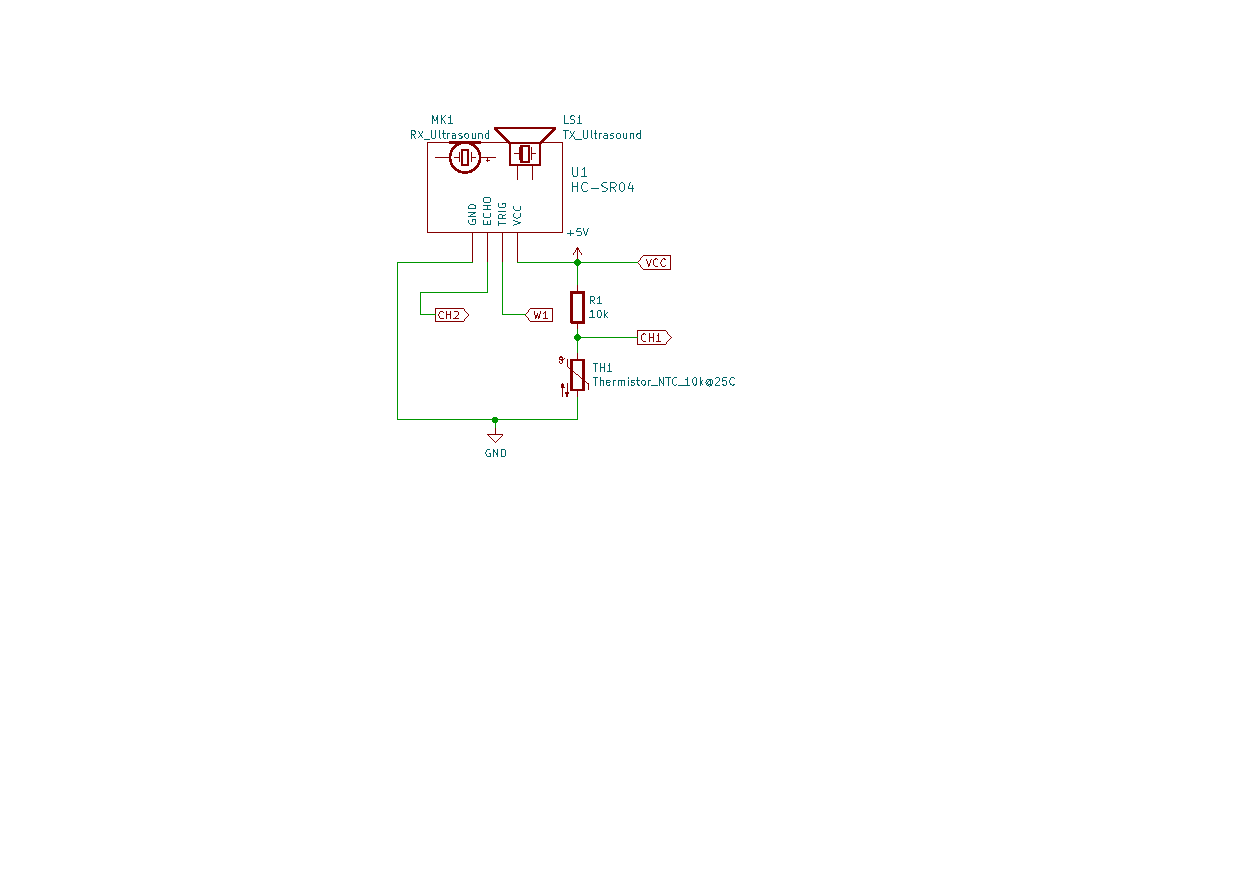
\includegraphics[scale=1]{schm}
    \caption{Schematica del circuito per la misurazione della velocità del suono e della temperatura
    \label{schm: mesctrl}}
\end{figure}

\subsection{Analisi del funzionamento del circuito}
Il componente principale è il Sensore HC-SR04, un sensore ad ultrasuoni che se utilizzato correttamente fornisce il tempo di viaggio (andata e ritorno) di un'onda sonora ad alta frequenza, sono udibile dall'uomo.
Questo componente deve essere alimentato da una tensione di 5 V; se al pin \verb+TRIG+ viene inviato un segnale di trigger (che deve soddisfare le condizioni di durata specifiche, vale a dire che l'impulso deve avere una durata superiore ai $10 \mu S$) il componente genera un segnale continuo alto nel pin \verb+ECHO+ e un'onda sonora che si propaga finché non incontra un ostacolo, per cui tornerà indietro e verrà captato dal sensore piezoelettrico,; a questo punto, il segnale alto presente nel pin \verb+ECHO+ tornerà ad essere basso. Controllando quindi quest'ultimo pin tramite l'oscilloscopio sarà possibile individuare un segnale della stessa durata che impiega l'onda sonora a propagarsi, riflettersi su un oggetto, e ritornare indietro.
\begin{figure}[H]
    \centering
	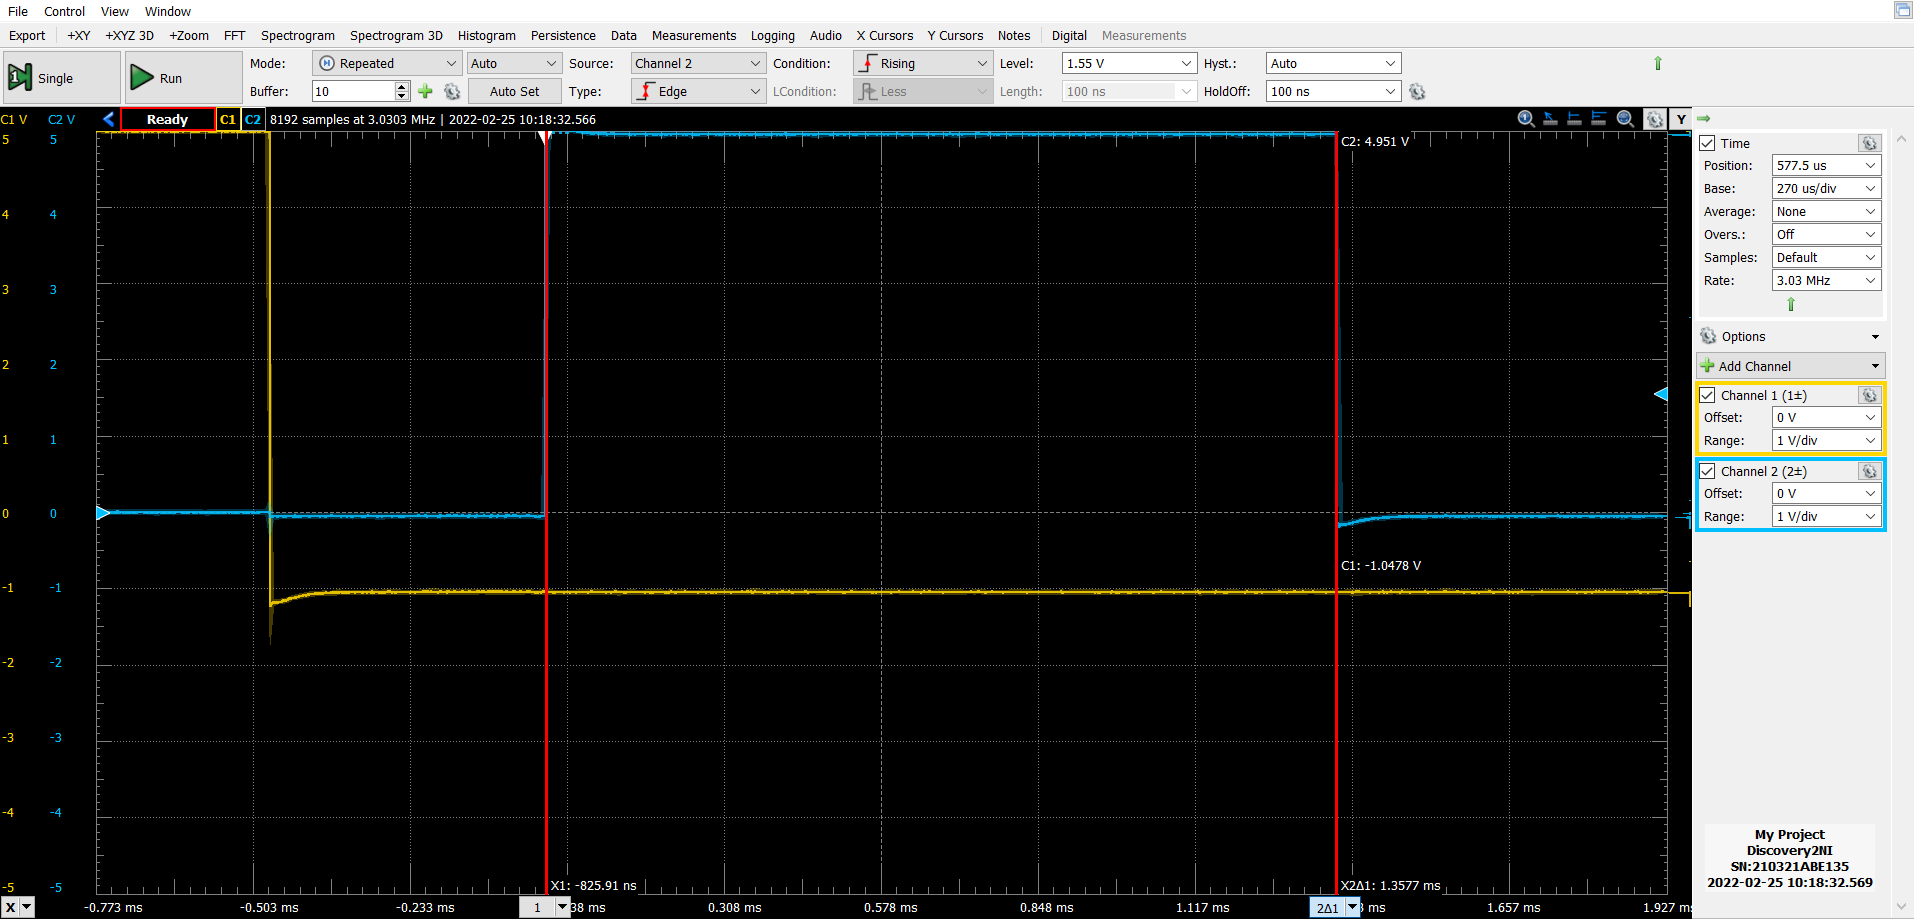
\includegraphics[scale=0.4]{echo}
    \caption{Segnali di Trigger (in giallo, su CH1) ed Echo (in blu, su CH2) per una misura con bersaglio a 15 cm di distanza}
\end{figure}
Inoltre è stato montato anche un sensore di temperatura tramite un partitore di tensione con una resistenza da $10 k\ohm$ e un termistore con $R_0 =10 k\ohm$, e misurando la tensione presente tra i due.
Conoscendo quindi la distanza D del sensore dell'oggetto, è possibile ricavare la velocità del suono come
\begin{equation}
v= \frac{2 D}{\Delta T}
\end{equation}
\subsection{Misura}
Si è proceduto con la misura di tempi di viaggio per diversi valori di distanza sensore oggetto. Successivamente abbiamo fatto un plot con python della distanza in funzione del tempo, facendo poi un fit lineare e ricavandone il coefficiente angolare e l'intercetta; In particolare si sono divise le situazioni di distanze corte (tra 15 e 25 cm) e distanze più lunghe (sopra i 25 cm).
\begin{table}[H]
\centering
\begin{tabular}{cc}
Travel Time [ms] & Distance [cm] \\
0.86 & 15   \\
0.92 & 16   \\
0.98 & 17   \\
1.03 & 18  \\
1.10 & 19   \\
1.15 & 20   \\
1.21 & 21   \\
1.27 & 22   \\
1.32 & 23  \\
1.39 & 24 
\end{tabular}
\caption{Tabella con distanze e tempi di viaggio impiegati nell'esperimento delle distanze brevi}
\end{table}
\begin{table}[H]
\centering
	\begin{tabular}{cc}
	\hline
	Travel Time [ms] & Travel Space [mm] \\ \hline
	1.44                              & 504                                  \\
	1.50                              & 524                                  \\
	1.56                              & 540                                  \\
	1.60                              & 564                                  \\
	1.65                              & 582                                  \\
	1.71                              & 600                                  \\
	1.74                              & 622                                  \\
	1.83                              & 644                                  \\
	1.88                              & 664                                  \\
	1.94                              & 682                                  \\
	2.00                              & 700                                  \\
	2.05                              & 720                                  \\
	2.11                              & 740                                  \\
	2.18                              & 756                                  \\
	2.23                              & 784                                  \\
	2.29                              & 800                                  \\
	2.33                              & 820                                  \\
	2.41                              & 840                                  \\
	2.47                              & 860                                  \\
	2.51                              & 880                                 
	\end{tabular}
	\caption{Tabella con spazi percorsi e tempi di viaggio impiegati nell'esperimento delle distanze lunghe}
\end{table}
\begin{figure}[H]
    \centering
	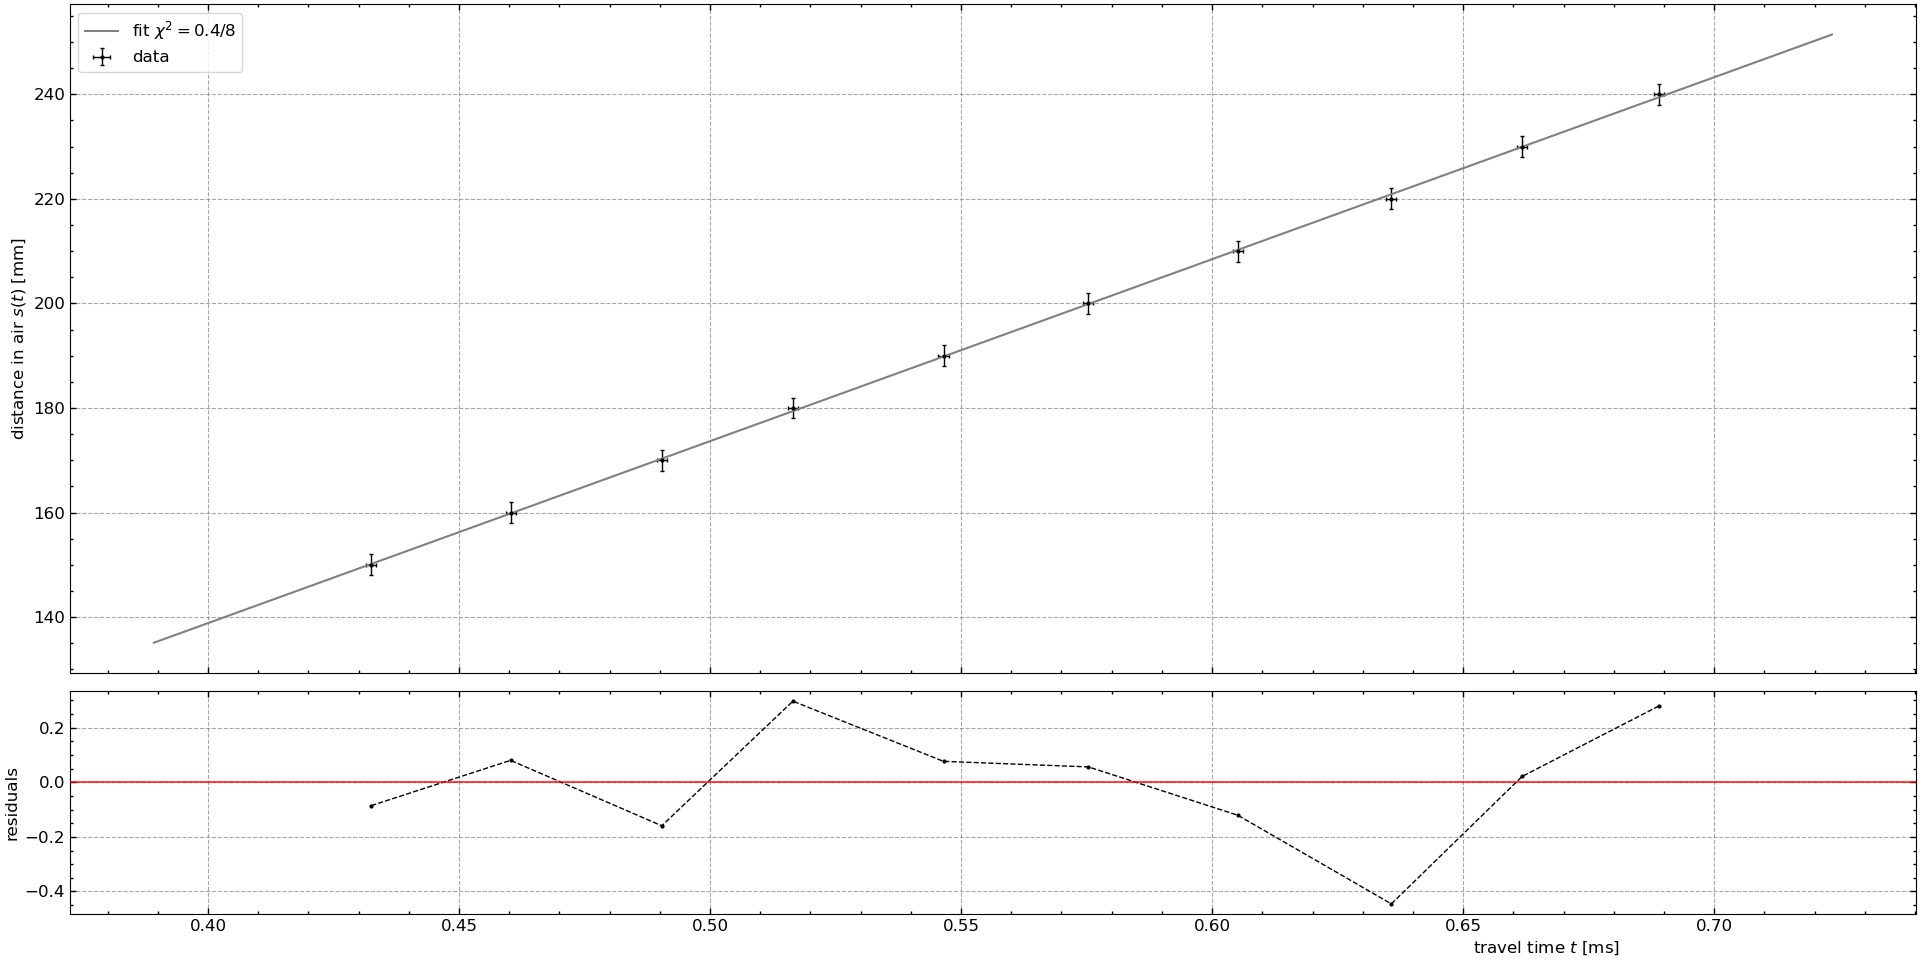
\includegraphics[scale=0.3]{2}
    \caption{Distanze corte in funzione del tempo}
\end{figure}
\begin{figure}[H]
    \centering
	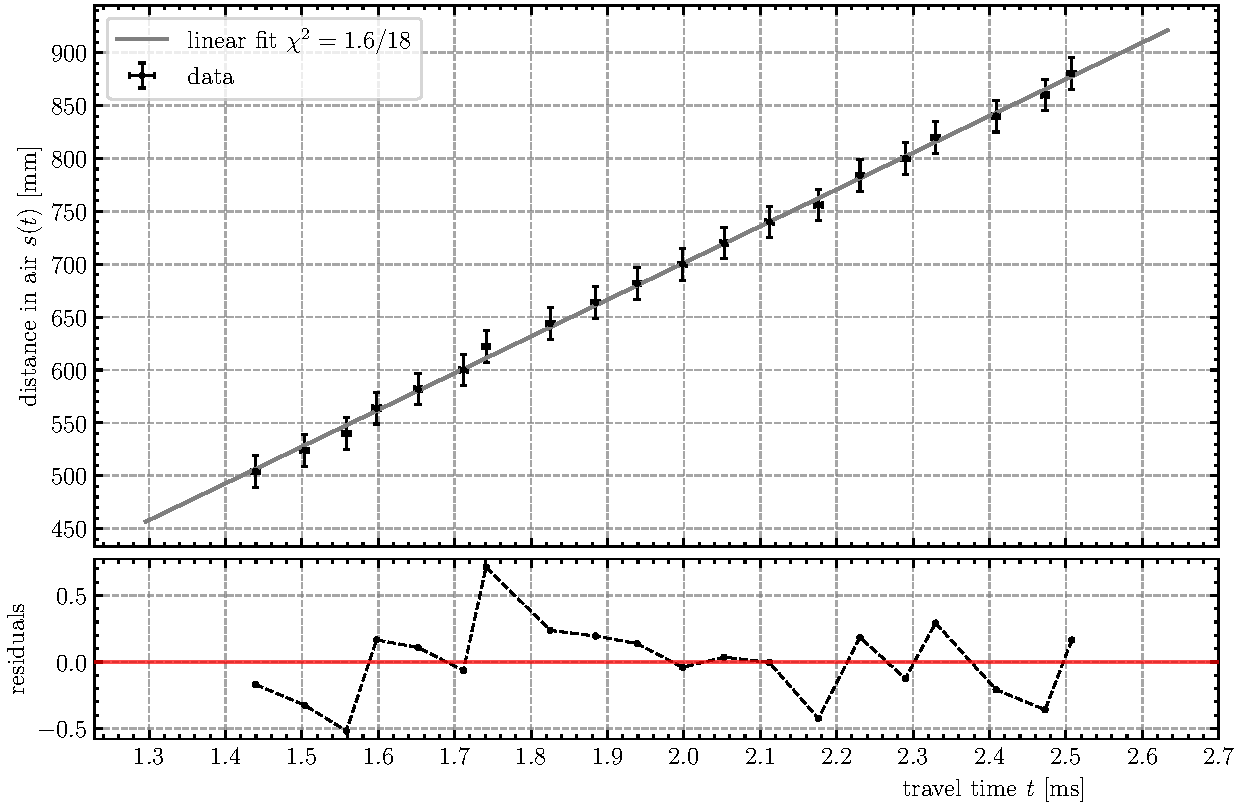
\includegraphics[scale=0.7]{railtime}
    \caption{Distanze lunghe in funzione del tempo}
\end{figure}
\begin{table}[H]
\centering
\begin{tabular}{cc|c}
\toprule
$V_s [\frac{m}{s}]$& $\sigma V_s$ & $Temperatura [Celsius]$ \\
\midrule
348.0 & 1.8 & 20\\
347.3 & 3.0 & 19\\
\bottomrule
\end{tabular}
\caption{Risultati del fit lineare per la velocità del suono}
\end{table}
In entrambi i casi abbiamo ottenuto anche un'intercetta che fosse compatibile con 0:
\begin{table}[H]
\centering
\begin{tabular}{cc}
\toprule
$q [\frac{m}{s}]$& $\sigma V_s$ \\
\midrule
-0.3 & 6.1 \\
-0.4 & 1.0 \\
\bottomrule
\end{tabular}
\caption{Risultati del fit lineare per la velocità del suono}
\end{table}
Nel primo caso (distanze brevi), per misurare correttamente la distanza, senza esagerare con l'errore associato, è stata ricavata la posizione del cristallo piezoelettrico inserendo un piccolo oggetto in carta (in modo da non danneggiare nulla) all'interno dei due occhi del sensore, da cui abbiamo ricavato che ci sono circa 5 mm di distanza tra il cristallo e la rete di protezione esterna. Per cui è stato possibile diminuire l'incertezza sulla distanza fino a 2 millimetri. Nell'altro esperimento invece è stata presa la distanza a partire dal punto medio dell'occhio, utilizzando come incertezza la metà dello spessore. Per quanto riguarda i tempi invece sono stati presi alla stessa maniera, utilizzando il metodo dei cursori sull'asse x e misurando la durata dell'impulso in \verb+ECHO+. I 2 esperimenti sono stati eseguiti all'interno di 2 case diverse in città diverse, quindi con condizioni di umidità relative diverse, nonostante ciò sono risultate perfettamente compatibili tra di loro, e con la velocità aspettata di $343 \frac{m}{s}$ a $20 \degree C$ entro le 3 barre di errore massime.
%=======================
\section{Dipendenza della velocità dalla temperatura}
Sappiamo che la velocità del suono attraverso l'aria non è costante ma varia, principalmente a causa della temperatura e dell'umidità.
Nel nostro caso proveremo a misurare questo cambiamento tramite un sensore detto termistore che varia la sua resistenza in funzione della temperatura.
Tramite un partitore di tensione possiamo misurare il potenziale compreso tra il una resistenza da 10 $k\ohm$ e il termistore per poi ricavarne il valore.
\begin{equation}
R_t=\frac{R_1V_2}{V_{cc}-V_2}
\end{equation}
Dove $V_2$ è la tensione misurata da CH1.
A quel punto sappiamo che la temperatura e la resistenza sono legati dall'equazione:
\begin{equation}
\frac{1}{T}= \frac{1}{T_0} + \frac{ln(\frac{R}{R_0})}{B}
\end{equation}
Inoltre la velocità del suono e la temperatura sono legati da:
\begin{equation}
V_s=v_0\sqrt{\frac{T+273.15}{273.15}}
\end{equation}
Dove T è la temperatura espressa in Celsius e $V_0$ la velocità del suono a 0 gradi Celsius.
\subsection{Misura}
Come prima, abbiamo misurato la durata dell'impulso ECHO a distanza fissa di $252 \pm 2 \; mm$ (anche in questo caso si è diminuita l'incertezza prendendo come punto di partenza delle onde 5 mm dalla fine dell'occhio del sensore) a diverse temperature, lasciando il circuito montato e fisso sempre nello stesso punto. Nonostante risulti semplice lasciare il circuito montato e funzionante, siamo riusciti a misurare un intervallo di solo $5 \degree C$ compresi tra i 15 e i 20; che sono stati comunque sufficienti per ricavare $v_0$. Abbiamo quindi preso le misure dei tempi tramite cursori sulle x misurando la durata dell'impulso di echo e dei valori di $V_2$ tramite la funzione VOLTMETER di Waveforms.
\begin{table}[H]
\centering
\begin{tabular}{ccc}
\toprule
Time [ms] & $V_2$ & Temperatura sul termostato \\
\midrule
1.49 & 3.11 & 15 \\
1.49 & 3.03 & 16 \\
1.48 & 2.98 & 17 \\
1.48 & 2.93 & 18 \\
1.47 & 2.88 & 19 \\
1.47 & 2.83 & 20
\end{tabular}
\caption{Tabella dei tempi di percorrenza in funzione della temperatura}
\end{table}
A questo punto abbiamo combinato le equazioni (2) e (3) per ricavare i dati di velocità e temperatura e le incertezze propagandole dalle medesime funzioni. In seguito si è condotto un fit con modello l'eq. (5) per ricavare $v_0$.
\begin{figure}[H]
    \centering
	\includegraphics[scale=0.3]{Temperature}
    \caption{Fit e residui per la velocità del suono in funzione della temperatura}
\end{figure}
Da qui abbiamo ottenuto che $v_0 =331 \pm 1 \; m/s$ che risulta essere perfettamente compatibile con il valore atteso. Ovviamente bisogna stare attenti a riportare le misure in uscita dall'equazione (3) in Celsius, altrimenti è sufficiente rivedere l'equazione (4).
%=======================
\section*{Conclusioni e commenti finali}
Si è riusciti a dare una misura ragionevole della velocità del suono in aria
e si è riusciti ad apprezzare la sua dipendenza dalla temperatura ambientale
con un semplice sensore ad ultrasuoni ed un termistore.

%=======================
\section*{Dichiarazione}
I firmatari di questa relazione dichiarano che il contenuto della relazione \`e
originale, con misure effettuate dai membri del gruppo, e che tutti i firmatari
hanno contribuito alla elaborazione della relazione stessa.


\end{document}
